\documentclass[8pt]{beamer}
\usepackage{tikz}
\usepackage[utf8]{vietnam}
\usepackage{amsmath}
\usepackage{graphicx}
\usepackage{mathrsfs}
\usepackage{amsmath,amsfonts,amsthm}
\usepackage{wrapfig}
\usepackage{hyperref}
\usetheme{Copenhagen}
\usecolortheme{spruce}
\setbeamertemplate{navigation symbols}{}
\setbeamertemplate{headline}{}
\setbeamertemplate{footline}{}
\title[Kết quả nghiên cứu tuần 0]
{Kết quả nghiên cứu tuần $0$}
\subtitle{Phòng thí nghiệm Thông tin Vô tuyến}
\author[Phòng thí nghiệm thông tin Vô tuyến]
{Tín Vũ}
\date[VLC 2021] % (optional)
{tinvu1309@gmail.com}
\begin{document}
\frame{\titlepage}
\begin{frame}{Mục lục}
\tableofcontents
\end{frame}
\begin{frame}{Tài liệu tham khảo}
\section{Tài liệu tham khảo}
Tài liệu tham khảo được sử dụng để nghiên cứu gồm: Calculus 7E (James Stewart), Fundamental of Physics (David Halliday, 10th)
\end{frame}
\begin{frame}{Giới thiệu các toán tử trong Giải tích vector}
\section{Giới thiệu các toán tử trong Giải tích vector}
\subsection{Toán tử $\nabla$}
\begin{itemize}
\item Toán tử $\nabla$
\end{itemize}
Ý tưởng của toán tử $\nabla$  bắt nguồn từ phép toán đạo hàm có hướng được mô tả như sau:
\begin{figure}[h]
			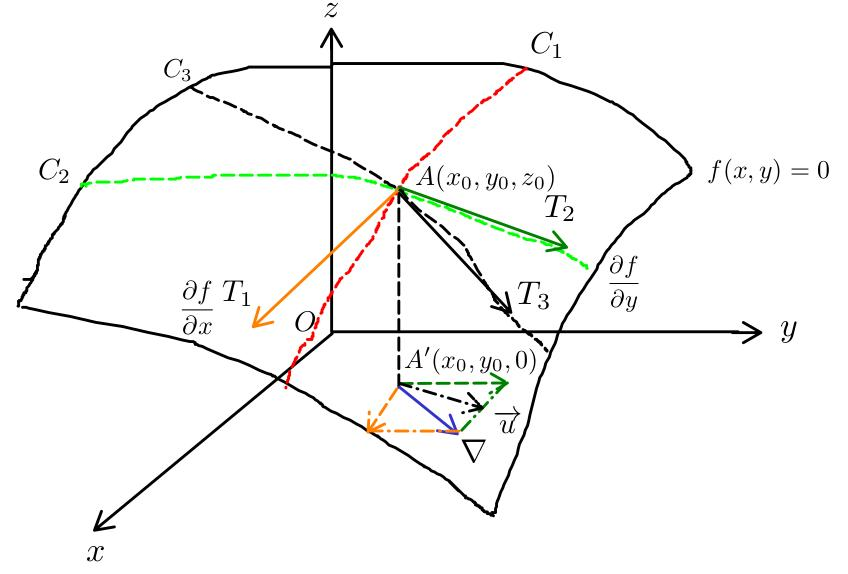
\includegraphics[width=0.8\textwidth]{nabla1.jpg}
			\caption{Directional derivative}			\label{fig:re1}
\end{figure}
\end{frame}
\begin{frame}{Giới thiệu các toán tử trong Giải tích vector}
	Ta định nghĩa đạo hàm có hướng tại tại điểm $A(x_{0},y_{0},f(x_{0},y_{0}))$ theo phương $\overrightarrow{u}=a\hat i+b\hat j$ với $\overrightarrow{u}$ là vector đơn vị như sau:
\begin{equation*}
	\begin{split}
		D_{\overrightarrow{u}}f(x_{0},y_{0})&=\lim_{h\to 0}\frac{f(x_{0}+ah,y_{0}+bh)-f(x_{0},y_{0})}{h}=\alert{a\frac{\partial f(x,y)}{\partial x}+b\frac{\partial f(x,y)}{\partial y}}\\
						    &=\alert{<a,b> \cdot \left<\frac{\partial f(x,y)}{\partial x}, \frac{\partial f(x,y)}{\partial y}\right>}
\end{split}
\end{equation*}
Về ý nghĩa hình học, giá trị đạo hàm vừa tính được ở trên chính là hệ số góc của tiếp tuyến $T_{3}$ của đường cong $C_{3}$. Nếu ta định nghĩa toán tử $\nabla$: $$\nabla=\frac{\partial f(x,y)}{\partial x}\hat i+\frac{\partial f(x,y)}{\partial y}\hat j$$ Ta có thể dễ dàng viết lại công thức đạo hàm có hướng như sau:
$$D_{\overrightarrow{u}}f(x_{0},y_{0})=\overrightarrow{u}\cdot \nabla$$
Từ kết quả trên, ta có thể thấy đường cong dốc nhất từ $A$ có hình chiếu $\overrightarrow{u}$ của nó \textbf{cùng phương} với $\nabla$, để đảm bảo $|D_{\overrightarrow{u}}f(x_{0},y_{0})| \text{ max}$.
\\ Tổng quát hóa, ta định nghĩa toán tử $\nabla$ cho 3 biến:
$$\alert{{\nabla}=\frac{\partial f(x,y,z)}{\partial x}\hat i+\frac{\partial f(x,y,z)}{\partial y}\hat y+\frac{\partial f(x,y,z)}{\partial z}\hat k}$$
\end{frame}
\begin{frame}{Giới thiệu các toán tử trong Giải tích vector}
Ta giới thiệu ứng dụng của toán tử $\nabla$ trong bài toán tìm cực trị có điều kiện (phương pháp nhân tử Lagrange) như sau: tìm cực trị của hàm số $f(x,y)$ với ràng buộc $g(x,y)=K$.
\begin{figure}[h]
			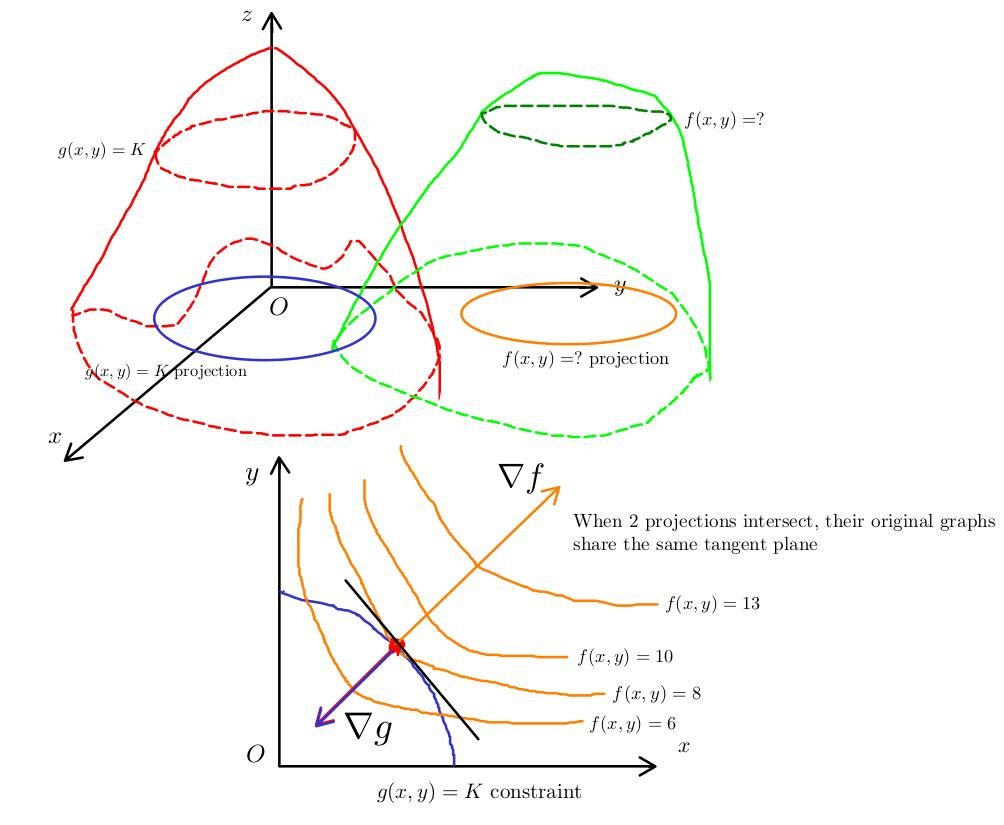
\includegraphics[width=0.7\textwidth]{graph.jpg}
			\caption{How to find Lagrange multiplier ?}			\label{fig:re2}
\end{figure}

\end{frame}
\begin{frame}{Giới thiệu các toán tử trong Giải tích vector}
Vậy ta cần giải hệ để tìm cực trị của hàm $f(x,y)$:
\begin{equation*}
\begin{cases}
	\nabla f(x,y)=\alert{\lambda}\nabla g(x,y)\\
	g(x,y)=K\\
\end{cases}
\end{equation*}
Tổng quát hóa, trong trường hợp ta muốn tìm cực trị của hàm $3$ hoặc nhiều biến hơn nữa:
\begin{equation*}
\begin{cases}
	\nabla f(x,y,z)=\alert{\lambda}\nabla g(x,y,z)\\
	g(x,y,z)=K\\
\end{cases}
\end{equation*}
Nếu có nhiều hơn $1$ ràng buộc, ta lần lượt thêm các nhân tử Lagrange $\mu$ vào phương trình Lagrange.
\begin{equation*}
\begin{cases}
	\nabla f(x,y,z)=\alert{\lambda}\nabla g(x,y,z)+\alert{\mu}\nabla h(x,y,z)\\
	g(x,y,z)=K\\
	h(x,y,z)=L\\
\end{cases}
\end{equation*}
 Đây là một kết quả cực mạnh dùng để tìm giá trị lớn nhất/nhỏ nhất của các hàm số đa biến rất dễ dàng mà không cần phải dùng bất đẳng thức sơ cấp.
\end{frame}
\begin{frame}{Giới thiệu các toán tử trong Giải tích vector}
Một trường vector (vector field) $\overrightarrow{F}$ được gọi là một \textbf{trường thế} (conservative vector field) khi và chỉ khi tồn tại vector thế $f$ (potential vector) thỏa mãn:
$$\overrightarrow{F}=\nabla f$$
Trường thế còn được gọi là \textbf{trường gradient}. Từ nguyên lý cơ sở của Giải tích vector: cho một đường cong $C$ bất kì có phương trình $\overrightarrow{r(t)}$ với $a\leq t\leq b$, giá trị tích phân đường của nó dọc theo đường cong trong trường gradient chỉ phụ thuộc vào điểm đầu và điểm cuối, hoàn toàn không phụ thuộc vào dạng đường cong $C$:
$$\int_{C}\nabla f \cdot d \overrightarrow{r}=f(\overrightarrow{r(b)})-f(\overrightarrow{r(a)})$$
Trong tự nhiên có 2 trường thế quan trọng là trường trọng lực (gravitational field) và điện trường (electric field).
\end{frame}
\begin{frame}{Giới thiệu các toán tử trong Giải tích vector}
\subsection{Toán tử curl}
\begin{itemize}
	\item Toán tử curl
\end{itemize}
Xét một trường vector $\overrightarrow{F}=P(x(t),y(t))\hat i+Q(x(t),y(t))\hat j$ và môt miền đơn liên kín $C$ có phương trình $\overrightarrow{r(t)}$ $(a\leq t\leq b)$ được biểu diễn như sau:
\begin{figure}[h]
			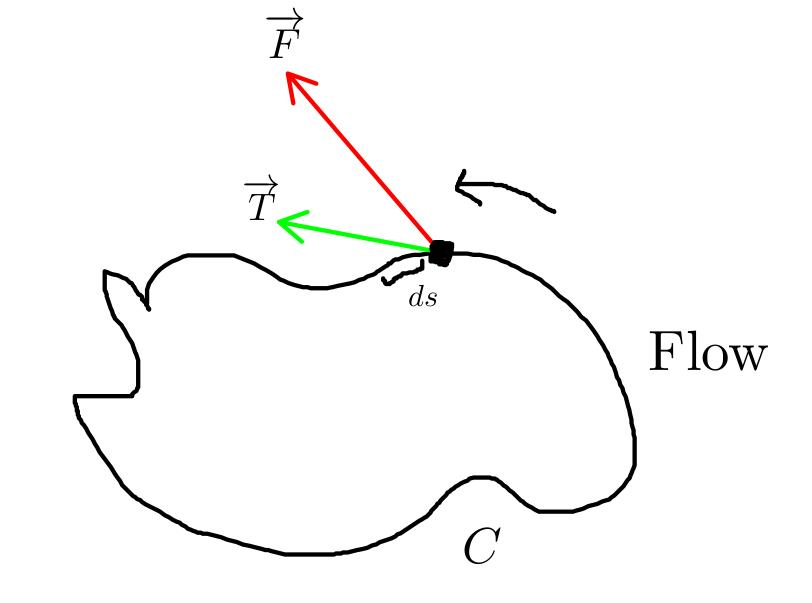
\includegraphics[width=0.4\textwidth]{flow.jpg}
			\caption{Example of flow}			\label{fig:re3}
\end{figure}
\begin{equation*}
	\textbf{Flow}=	\oint_{C}\overrightarrow{F}\overrightarrow{T}ds=\oint_{C}\overrightarrow{F}d\overrightarrow{r}=\int_{C}P(x,y)dx+Q(x,y)dy
\end{equation*}
Từ kết quả của định lý Green, nếu ta kí hiệu $R$ (region bounded by curve $C$), ta có:
$$\textbf{Flow}=\oint_{C}\overrightarrow{F}\overrightarrow{T}ds=\iint_{R}\left(\frac{\partial Q(x,y)}{\partial x}-\frac{\partial P(x,y)}{\partial y}\right)dA$$
\end{frame}
\begin{frame}{Giới thiệu các toán tử trong Giải tích vector}
Đại lượng trên chính là một trường hợp riêng của curl trong không gian 2 chiều. Tổng quát hóa, nếu ta có trường vector $F(x,y,z)=P(x,y,z)\hat i + Q(x,y,z)\hat j + R(x,y,z)\hat k$, ta xây dựng công thức của curl như sau (ta tạm thời thay kí hiệu $P(x,y,z)$ thành $P$):
$$\text{curl}\overrightarrow{F}=\left(\frac{\partial R}{\partial y}-\frac{\partial Q}{\partial z}\right)\hat i+\left(\frac{\partial P}{\partial z}-\frac{\partial R}{\partial x}\right)\hat j+\left(\frac{\partial Q}{\partial x}-\frac{\partial P}{\partial y}\right)\hat k=\alert{\nabla \times \overrightarrow{F}}$$
Ta viết lại định lý Green dưới dạng vector:
$$\textbf{Flow}=\oint_{C}\overrightarrow{F}\overrightarrow{T}ds=\iint_{R}(\text{curl} \overrightarrow{F})\cdot \hat k dA$$
\end{frame}
\begin{frame}{Giới thiệu các toán tử trong Giải tích vector}
\subsection{Toán tử div}
\begin{itemize}
	\item Toán tử div
\end{itemize}
Xét một trường vector $\overrightarrow{F}=P(x(t),y(t))\hat i+Q(x(t),y(t))\hat j$ và môt miền đơn liên kín $C$ có phương trình $\overrightarrow{r(t)}$ $(a\leq t\leq b)$ được biểu diễn như sau:

\begin{figure}[h]
			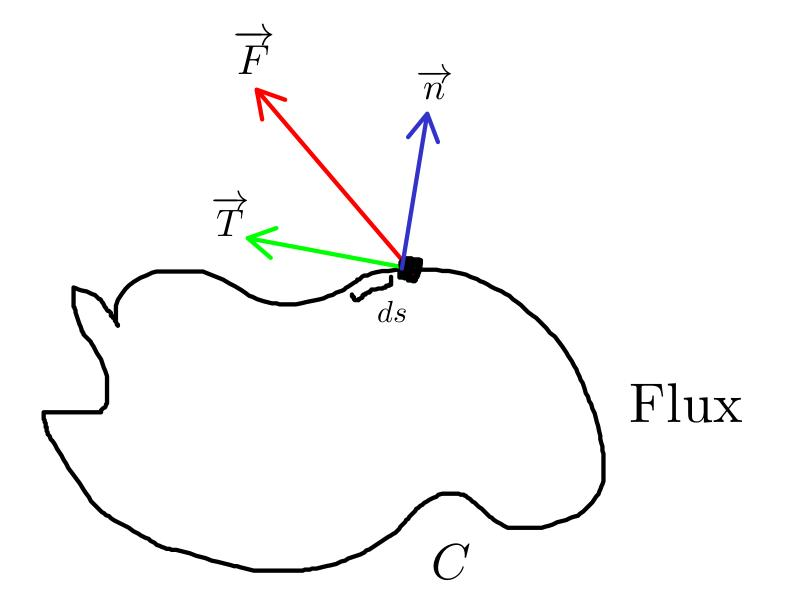
\includegraphics[width=0.4\textwidth]{flux.jpg}
			\caption{Example of flux}			\label{fig:re4}
\end{figure}
\begin{equation*}
\begin{split}
	\textbf{Flux}&=\oint_{C}\overrightarrow{F}\overrightarrow{n}ds=\oint_{C}\overrightarrow{F}(\overrightarrow{T}\times \hat k)ds=\oint_{C}\overrightarrow{F}\left(\frac{dy}{ds}\hat i-\frac{dx}{ds}\hat j\right)ds\\&=\int_{C}P(x,y)dy-Q(x,y)dx
\end{split}
\end{equation*}
\end{frame}
\begin{frame}{Giới thiệu các toán tử trong Giải tích vector}
Từ kết quả của định lý Green, nếu ta kí hiệu $R$ (region bounded by curve C), ta có:
\begin{equation*}
	\textbf{Flux}=\oint_{C}\overrightarrow{F}\overrightarrow{n}ds=\iint_{R}\left(\frac{\partial P(x,y)}{\partial x}+\frac{\partial Q(x,y)}{\partial y}\right)dA
\end{equation*}
Đại lượng trên chính là một trường hợp riêng của div trong không gian 2 chiều. Tổng quát hóa, nếu ta có trường vector $F(x,y,z)=P(x,y,z)\hat i + Q(x,y,z)\hat j + R(x,y,z)\hat k$, ta xây dựng công thức của div như sau (ta tạm thời thay kí hiệu $P(x,y,z)$ thành $P$):
$$\text{div}\overrightarrow{F}=\frac{\partial P}{\partial x}+\frac{\partial Q}{\partial y}+\frac{\partial R}{\partial z}=\alert{\nabla\cdot \overrightarrow{F}}$$
Ta viết lại định lý Green dưới dạng vector:
$$\textbf{Flux}=\oint_{C}\overrightarrow{F}\overrightarrow{n}ds=\iint_{R}\textbf{div}\overrightarrow{F}(x,y)dA$$
\end{frame}
\begin{frame}{Phương trình Maxwell và sóng điện từ}
\section{Phương trình Maxwell và sóng điện từ}
\begin{itemize}
\item Phương trình Maxwell
\end{itemize}
\subsection{Phương trình Maxwell}
\subsubsection{Định luật Gauss cho điện trường}
\begin{itemize}
\item[-]  Định luật Gauss cho điện trường
\end{itemize}
\begin{figure}[h]
			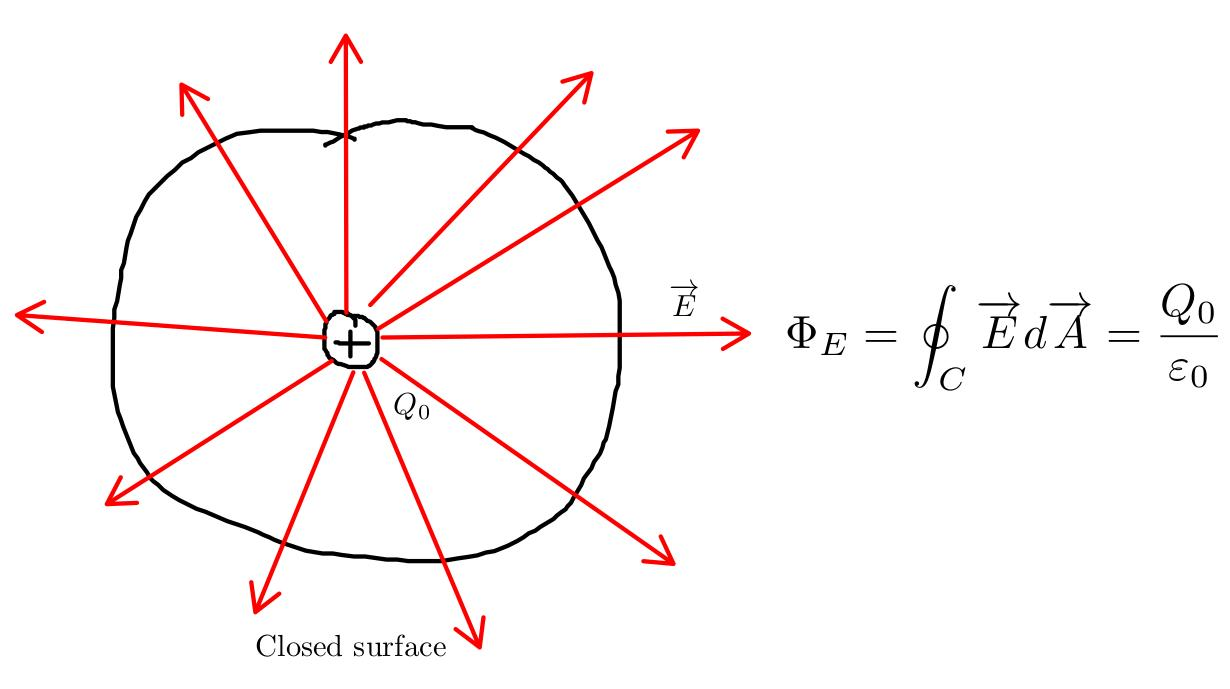
\includegraphics[width=0.5\textwidth]{gauss.jpg}
			\caption{Gauss's Law for Electric field}			\label{fig:re5}
\end{figure}
\subsubsection{Định luật Gauss cho từ trường}
\begin{itemize}
	\item[-] Định luật Gauss cho từ trường
\end{itemize}
\begin{figure}[h]
			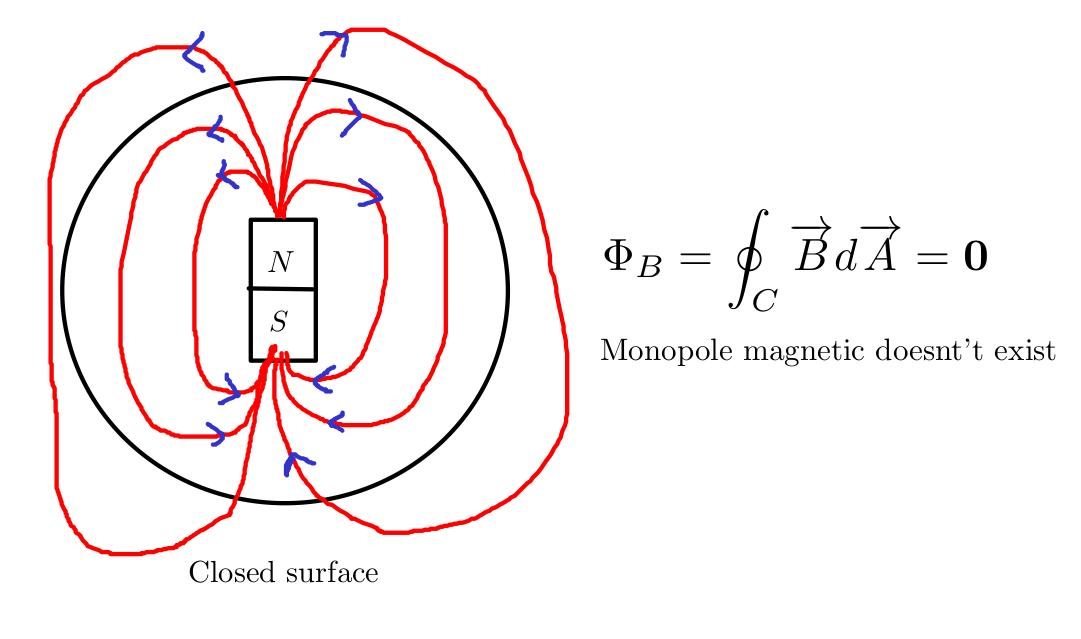
\includegraphics[width=0.4\textwidth]{mag.jpg}
			\caption{Gauss's Law for Magnetic field}			\label{fig:re6}
		\end{figure}
\end{frame}
\begin{frame}{Phương trình Maxwell và sóng điện từ}
\subsubsection{Định luật Faraday}
\begin{itemize}
	\item[-] Định luật Faraday
\end{itemize}
\begin{figure}[h]
			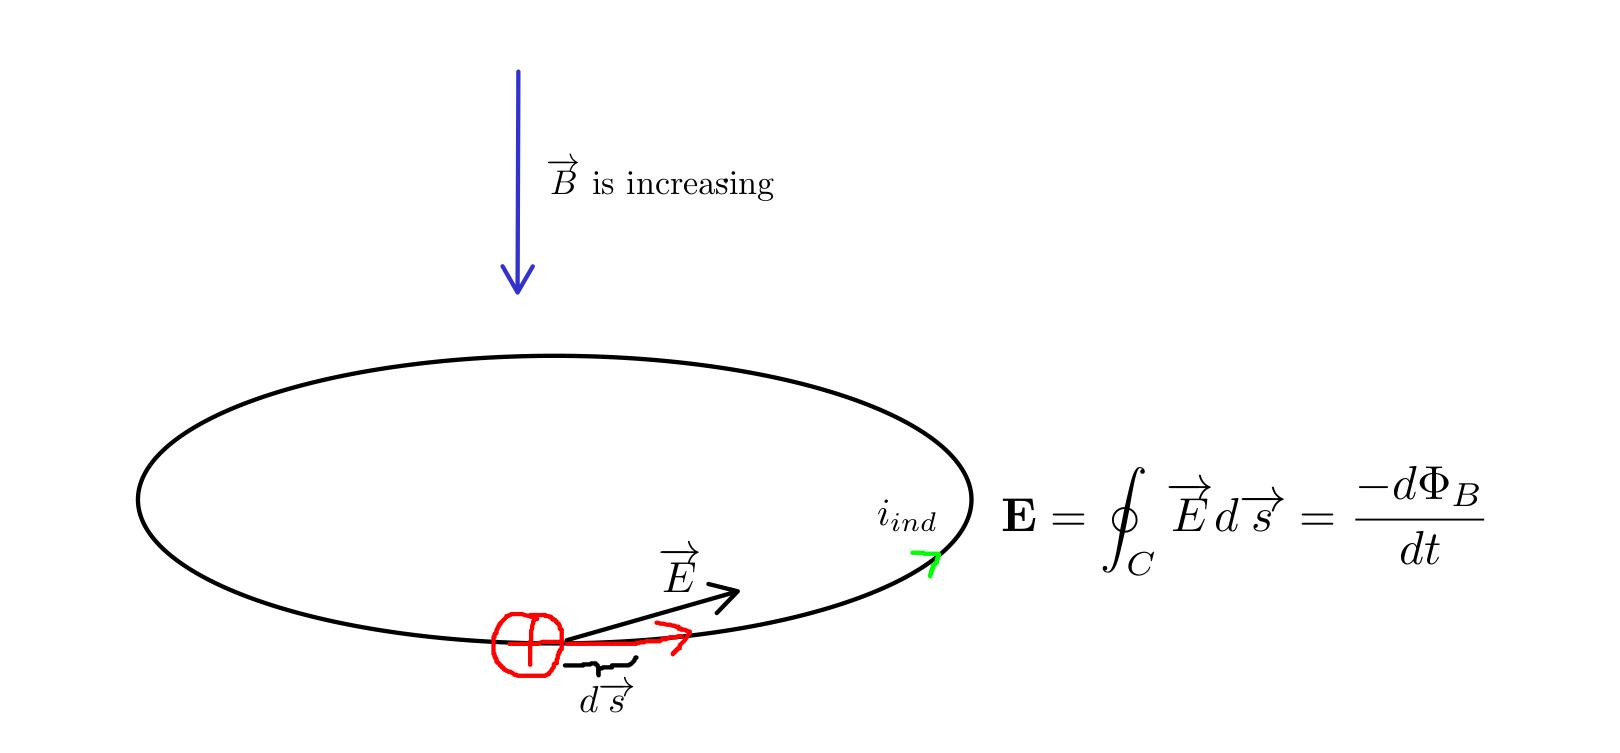
\includegraphics[width=0.9\textwidth]{faraday.jpg}
			\caption{Faraday's Law}			\label{fig:re7}
		\end{figure}

\end{frame}
\begin{frame}{Phương trình Maxwell và sóng điện từ}
\subsubsection{Định luật Maxwell-Ampere}
\begin{itemize}
\item[-] Định luật Ampere
\end{itemize}
\begin{figure}[h]
			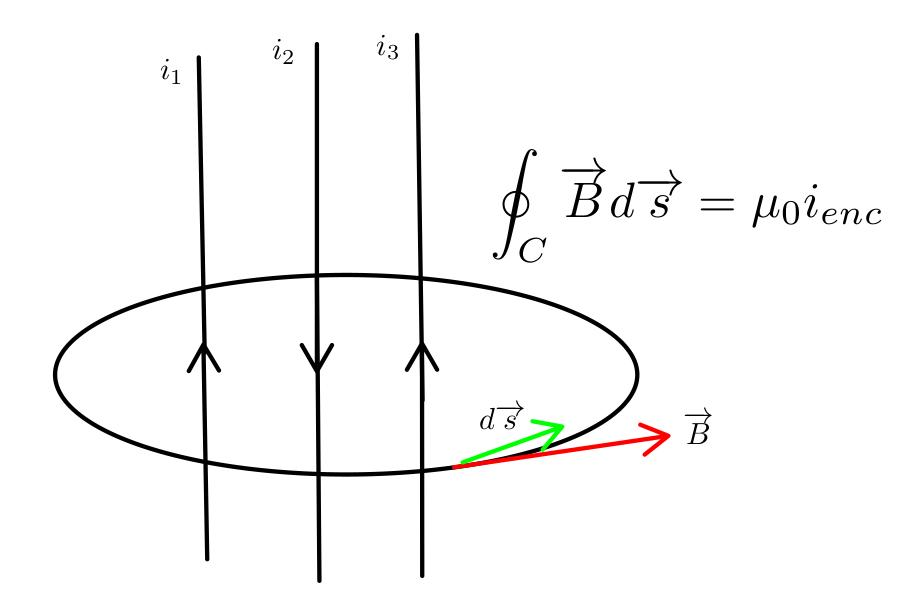
\includegraphics[width=0.7\textwidth]{ampere.jpg}
			\caption{Ampere's Law}\label{fig:re8}
		\end{figure}


\end{frame}
\begin{frame}{Phương trình Maxwell và sóng điện từ}
	Maxwell đã phát triển định luật Ampere thành định luật Maxwell-Ampere dựa trên hiện tượng giữa 2 bản tụ điện phẳng, thay đổi điện thông $\Phi_{E}$ và quan sát từ trường $\overrightarrow{B}$ xuất hiện như sau:
\begin{figure}[h]
	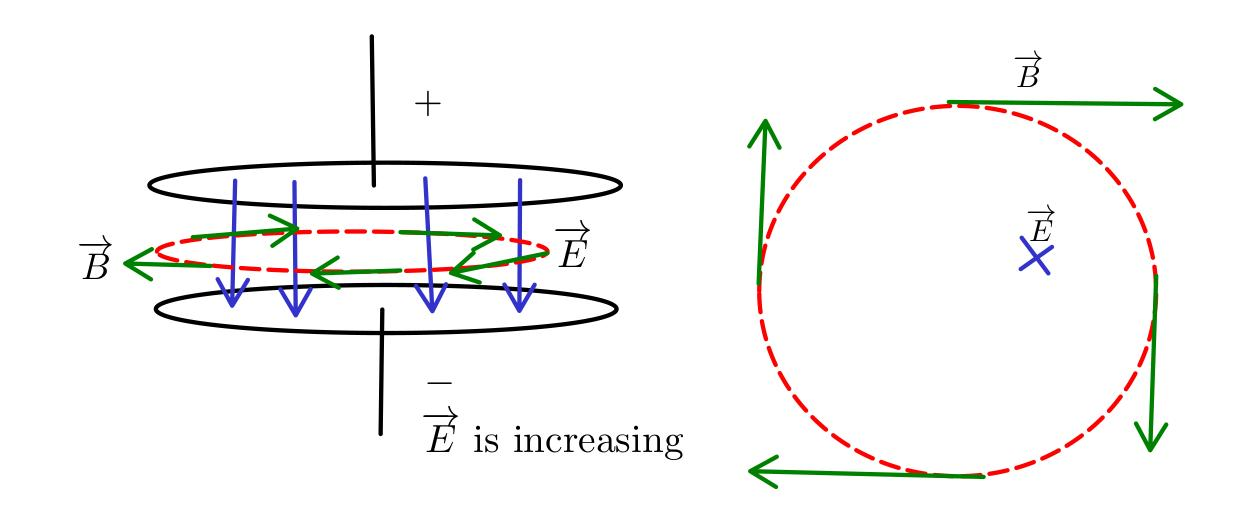
\includegraphics[width=0.7\textwidth]{maxwell.jpg}
			\caption{Ampere's Law}\label{fig:re9}
		\end{figure}
		Ta có thể thấy rằng, giữa hai mặt phẳng tụ có một dòng điện ảo (displacement current), không phải dòng điện vật lý thực, được hình thành bởi sự biến thiên lượng điện tích trong quá trình sạc tụ, ta gọi dòng điện này là $i_{dis}$. Vậy với tác nhân $2$ dòng điện gây ra từ trường $\overrightarrow{B}$, ta có phương trình Ampere dạng mở rộng (Ampere-Maxwell equation) như sau:
\end{frame}
\begin{frame}{Phương trình Maxwell và sóng điện từ}
\begin{equation*}
\begin{split}
	\oint_{C}\overrightarrow{B}d\overrightarrow{s}=\mu_{0} i_{enc}+\mu_{0}i_{dis}=\mu_{0}i_{enc}+\mu_{0}\frac{dq}{dt}=\mu_{0}i_{enc}+\mu_{0}\frac{\varepsilon_{0}d\Phi_{E}}{dt}
\end{split}
\end{equation*}
 Vậy tổng hợp lại, ta thu được $4$ phương trình Maxwell ở dạng tích phân:
 \begin{block}{Phương trình Maxwell ở dạng tích phân}
\begin{enumerate}
	\item $$\Phi_{E}=\oint_{C}\overrightarrow{E}d\overrightarrow{A}=\frac{Q_{0}}{\varepsilon_{0}}$$
	\item $$ \Phi_{B}=\oint_{C}\overrightarrow{B}d\overrightarrow{A}=0$$
	\item $$\mathscr{E}=\oint_{C}\overrightarrow{E}d\overrightarrow{s}=\frac{-d\Phi_{B}}{dt}$$
	\item $$\oint_{C}\overrightarrow{B}d\overrightarrow{s}=\mu_{0}i_{enc}+\mu_{0}\varepsilon_{0}\frac{d\Phi_{E}}{dt}$$
\end{enumerate}
\end{block}
\end{frame}
\begin{frame}{Phương trình Maxwell và sóng điện từ}
Ta cũng thu được phương trình Maxwell ở dạng vi phân với các toán tử đã giới thiệu ở trên:
\begin{block}{Phương trình Maxwell ở dạng vi phân}
\begin{enumerate}
	\item $$\nabla\cdot\overrightarrow{E}=\frac{\rho}{\varepsilon_{0}}$$
	\item $$\nabla \cdot \overrightarrow{B}=0$$
	\item $$\nabla \times \overrightarrow{E}=-\frac{\partial \overrightarrow{B}}{\partial t}$$
	\item $$\nabla \times \overrightarrow{B}=\mu_{0}\overrightarrow{J}+\mu_{0}\varepsilon_{0}\frac{\partial \overrightarrow{E}}{\partial t}$$
\end{enumerate}
\end{block}
\end{frame}
\begin{frame}{Phương trình Maxwell và sóng điện từ}
\subsection{Sóng điện từ}
\begin{itemize}
\item Sóng điện từ
\end{itemize}
Ta quan sát hiện tượng vật lý sau: một điện tích dương $Q_{0}$ đang dao động qua lại trên một đoạn dây dẫn:

\begin{figure}[h]
	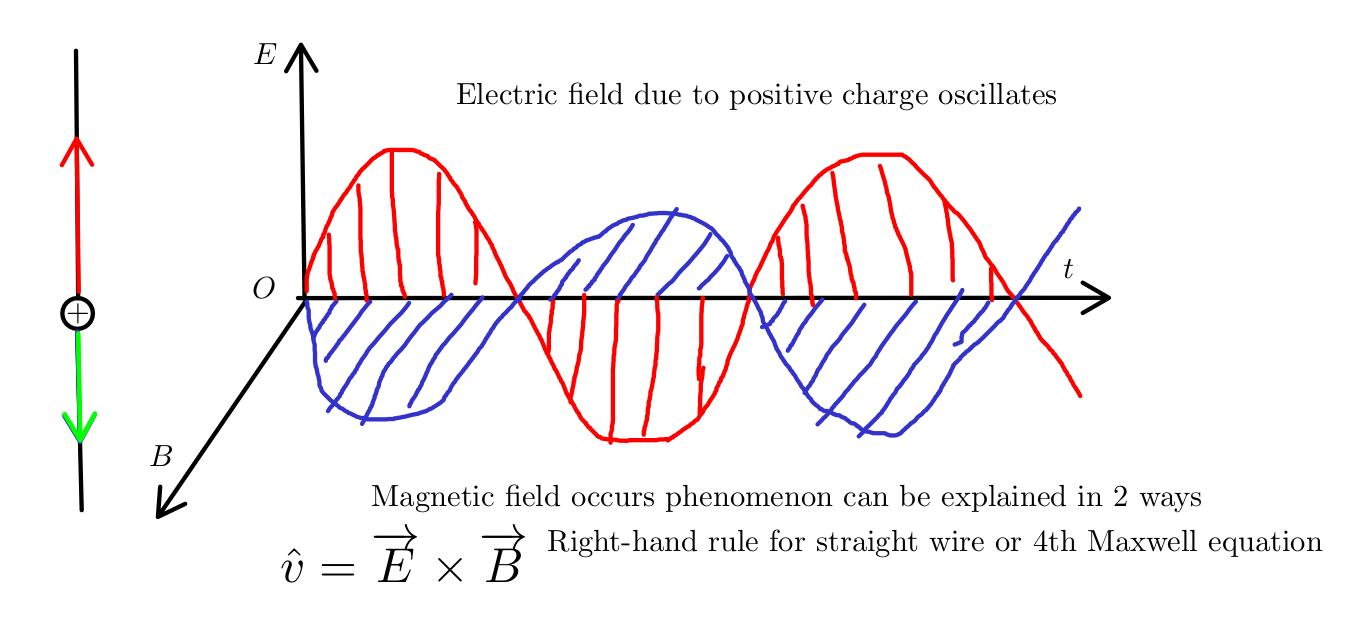
\includegraphics[width=0.9\textwidth]{wave.jpg}
			\caption{Electromagnetic wave}\label{fig:re10}
		\end{figure}
\end{frame}
\begin{frame}{Phương trình Maxwell và sóng điện từ}
Bằng cách áp dụng phương trình Maxwell 3 và 4, ta có thể dễ dàng nghiệm lại được kết quả tốc độ truyền sóng điện từ bằng tốc độ ánh sáng $c$ và $E=Bc$.
\\ Năng lượng của sóng điện từ được tính bằng độ lớn của vector Poynting:
$$\overrightarrow{S}=\frac{1}{\mu_{0}}\overrightarrow{E}\times\overrightarrow{B}$$

\begin{figure}[h]
			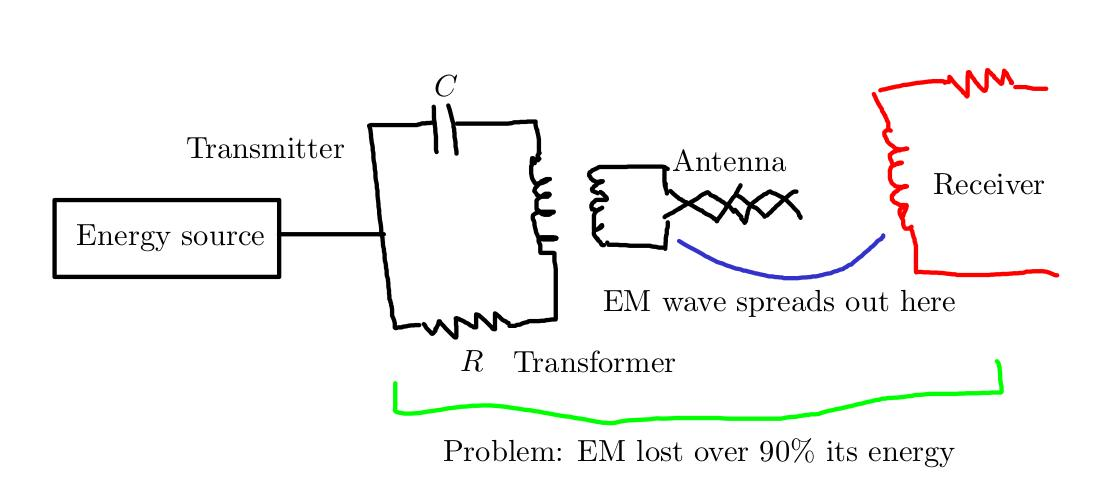
\includegraphics[width=0.7\textwidth]{antenna.jpg}
			\caption{Antenna simple block diagram}\label{fig:re10}
		\end{figure}
\textbf{Hướng nghiên cứu: thiết kế antenna có gain cực lớn để khắc phục vấn đề hao hụt năng lượng khi truyền trong không khí.}
\end{frame}
\begin{frame}{Hướng nghiên cứu tiếp theo}
\section{Hướng nghiên cứu tiếp theo}
Học nốt tích phân mặt, định lý Stoke (tham khảo Calculus 7E).
\\ Bổ túc kiến thức sóng EM nâng cao (tham khảo YouTube).
\\Bắt đầu đọc sách chuyên ngành về antenna (tham khảo Antenna Theory).
\end{frame}
\end{document}
